%!TEX root = ../AliPubV0JetspPb.tex

\section{\lda\ (\alda) and \ks\ reconstruction}

The reconstruction the \Vzero particles (\ks\, \lda, and \alda) follows (is fully consistent with) the analysis in \cite{Abelev:2013haa} with the exception of the rapidity selection of the particles and their the decay products.

\ask{See how much details is needed - since all follows from \cite{Abelev:2013haa}.}

Charged-hadron identification in the central barrel was performed with
the ITS, TPC and TOF detectors. The drift and strip layers
of the ITS provide a measurement of the specific energy loss with a
resolution of about 10\%. In a standalone tracking mode, the
identification of pions, kaons, and protons is thus extended down to
respectively 0.1, 0.2, 0.3 \gevc\ in \pt. The TPC provides particle
identification at low momenta via specific energy loss \dedx\ in the
fill gas by measuring up to 159 samples per track with a resolution of
about 6\%. The separation power achieved in \pPb\ collisions is
identical to that in pp collisions~\cite{Abelev:2014ffa}. Further outwards at about 3.7 m
from the beam line, the TOF array allows identification at higher \pt\
measuring the particle speed with the time-of-flight technique. The
total time resolution is about 85 ps for events in the multiplicity
classes from 0\% to $\sim 80$\%.  In more peripheral collisions, where
multiplicities are similar to pp, it decreases to about 120 ps due to
a worse start-time (collision-time) resolution~\cite{Abelev:2014ffa}.
The start-time of the event was determined by combining the time estimated using the particle arrival
times at the TOF and the time measured by the T0 detector.

Since the \pPb\ center-of-mass system moved in the laboratory frame
with a rapidity of \ynn\ = $-0.465$, the nominal acceptance of the
central barrel of the ALICE detector was asymmetric with respect to
\ycms\ = 0.  In order to ensure good detector acceptance and optimal
particle identification performance, tracks were selected in the
rapidity interval $0 < \ycms < 0.5$ in the nucleon-nucleon
center-of-mass system. Event generator studies and repeating the
analysis in $\left|\ycms\right| < 0.2$ indicate differences between
the two rapidity selections smaller than 2\% in the
normalization and 3\% in the shape of the transverse momentum
distributions.

The \pt\ differential yields of \Vzero particles were extracted via the invariant mass method described in \cite{Abelev:2013haa}. Table \ref{tab:v0cuts} presents the topological cuts applied on the candidate tracks of the decays daughters.

\begin{table}[t]
  \centering
  \begin{tabular*}{\linewidth}{@{\extracolsep{\fill}}lr}
    \hline
    &\\[-0.7em]
    Selection variable & Cut value \\[0.3em]
    \hline
    &\\[-0.7em]
    2D decay radius & $>0.50$~cm \\[0.3em]
    Daughter track DCA to prim. vertex & $>0.06~$cm \\[0.3em]
    DCA between daughter tracks & $<1.0~\sigma$ \\[0.3em]
    Cosine of pointing angle (\kzero) & $>0.97$ \\[0.3em]
    & ($<1\%$ signal loss) \\[0.3em]
    Cosine of pointing angle (\lmb\ and \almb) & $>0.995$ \\[0.3em]
    & ($<1\%$ signal loss) \\[0.3em]
    Proper lifetime (\kzero) & $<20$~cm \\[0.3em]
    Proper lifetime (\lmb\ and \almb) & $<30$~cm \\[0.3em]   
    \kzero\ mass rejection window (\lmb\ and \almb) & $\pm 10$~\mevc\ \\[0.3em]
    \lmb\ and \almb\ mass rejection window (\kzero) & $\pm 5$~\mevc\ \\[0.3em]
    \hline
  \end{tabular*}
  \caption{\vzero\ topological selection cuts (DCA: distance-of-closest approach). \ask{check if the cos theta \pt\ dependent(?)}}
  \label{tab:v0cuts}
\end{table}

Note, that the selection cuts for primary particle tracks used for the jet reconstruction are not compatible with the \Vzero\ candidate tracks. Consequently, the set of tracks used for the jet reconstruction and \Vzero\ candidates are not the same and the \Vzero\ particles are matched to a hard scattering by selecting their distance in the pseudo-rapidity and azimuthal angle plane. \ask{say what fraction}

\subsection{$\Vzero-$jet matching}
\label{sec:c05V0JetMat}

The yield of $\Vzero$ partincles associated to a hard scatterings (JC $\Vzero$) tagged by a jet within a cone $R$ was done in following steps:
\begin{itemize}
\item the \Vzero\ candidates are selected with the cuts defined within the acceptance of $|\eta|<0.75$;
\item the candidates are associated to the hard scattering with a distance cut in pseudo-rapidity and azimuthal angle plane ($\hlab \times \varphi)$: $\Delta R_{\Vzero-{\rm jet}}<R$, where
\begin{equation}
\Delta R_{\Vzero-{\rm jet}}=\sqrt{(\hlab^{\rm jet} - \hlab^{\Vzero})^{2} - (\varphi^{\rm jet} - \varphi^{\Vzero})^{2}}
\end{equation}
is the distance between the particle candidate and jet axis;
\item for each \pt\ interval of the \Vzero\ candidates matching at least one jet within the radius $R$ an invariant mass distribution \ask{(needs a demo figure?)} is constructed and the combinatorial background interpolated from the yield in side bands around the mass peak region defined by the width and mean of the peak for the inclusive \Vzero\ candidates;
\item finally, the JC yield is corrected for the contribution of particles from the underlying event (UE) (various estimators of \Vzero\ particles of the UE are discussed in subsection \ref{sec:V0UE}).
\end{itemize}

\begin{figure}[]
\begin{center}
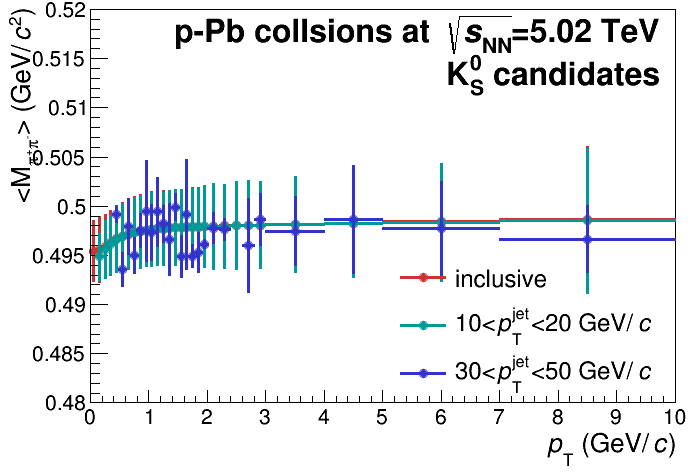
\includegraphics[width=.49\textwidth]{c04V0Reconstruction/KshortInvM}
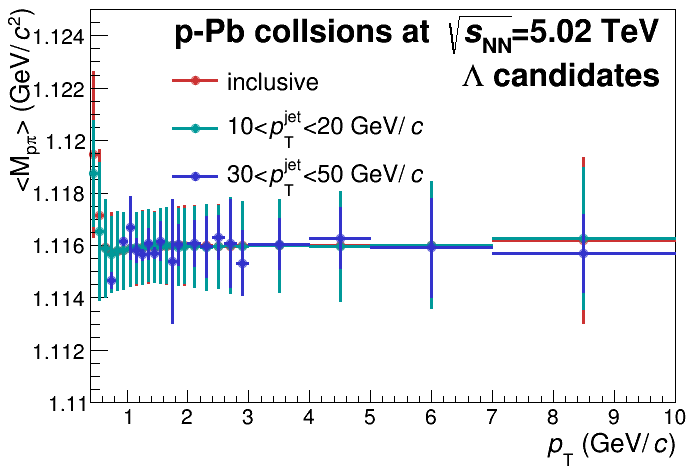
\includegraphics[width=.49\textwidth]{c04V0Reconstruction/LambdaInvM}
\caption{The mean and width of \Vzero\ invariant mass distribution extracted
         by the Gaussian fit for the inclusive $\Vzeros$ candidates
         and JC $\Vzero$ candidates as a function of $\pT$ in data.}
\label{fig:V0FitInvM}
\end{center}
\end{figure}

Figure~\ref{fig:V0FitInvM} shows the comparison of the mean and width of \Vzero\ invariant mass distribution extracted by the Gaussian fit for the inclusive \Vzeros\ candidates and JC \Vzero\ candidates as a function of $\pT$ in data.
The mean and width in the $\Vzero$ invariant mass distributions for the inclusive \Vzeros\ and JC \Vzeros\ are compatible within statistical uncertainties.
To avoid statistic fluctuations found in high-\pT\ jet selection, the number of JC \Vzeros is extracted using the mean and width obtained in the inclusive $\Vzero$ invariant mass distribution.

%%%%%%%%%%%%%%%%%%%%%%%%%%%%%%%%%%%%%%%%%%%%%%%%%%%%%%%%%%%%%%%%%%
\subsection{\Vzero\ particles from underlying event}
\label{sec:V0UE}

In order to measure the \Vzero\ yields in the underlying event (UE) (not associated to the hard scatterings tagged by the charged jets considered in this analysis) several estimators have been investigated:
\begin{itemize}
  \item the OC selection: the \Vzero\ particles that were not matched to any jet considered in the analysis within events containing a jet such that $\Delta R_{\Vzero-{\rm jet}} > R_{\rm cut}$;
  \item the PC selection: the \Vzero\ particles found in the perpendicular region (in the transverse plane) at angles larger than $\Delta \varphi = \varphi^{\rm jet} - \varphi^{\Vzero} > R_{\rm cut}$ \ask{(say the value)}
  \item the NJ selection: the \Vzero particles found in events that do not contain a jet with $\ptjet>5 \gevc$.
\end{itemize}

In practice, a useful quantity for performing the subtraction of the non-jet contribution of the \Vzero\ particles is their density per unit area $\rho^{\Vzero}(\pt)=N^{\Vzero}/A^{\Vzero}(\pt)$, where $A^{\Vzero}$ is the acceptance in pseudo-rapidity and azimuthal angle. Consequently, the number of the UE \Vzero\ particles within a jet can be calculated as $N=\rho^{\Vzero} \Ajet$ for each estimator separately. Note, in this analysis we consider the jet area \Ajet\ to be $\pi R^2$.

%%%%%%%%%%%%%%%%%%%%%%%%%%%%%%%%%%%%%%%%%%%%%%%%%%%%%%%%%%%%%%%%%%
\subsection{Efficiency}
\label{sec:c05V0EffiMC}

The efficiencies of \Vzero particles were estimated using DPMJET Monte Carlo generator \cite{Roesler:2000he} with the same cuts as in the data except the daughter track PID with ${\rm d}E/{\rm d}x$ in TPC. 
Figure~\ref{fig:c05EffiIncV0s} shows the efficiency of the inclusive $\Vzeros$ as a function of $\pT$ in three event multiplicity bins. For each of the event multiplicity class the efficiency is compared to the efficiency in minimum-bias events and it is found that the efficiency of inclusive $\Vzeros$ is independent on the event multiplicity.

\begin{figure}[htb]
\begin{center}
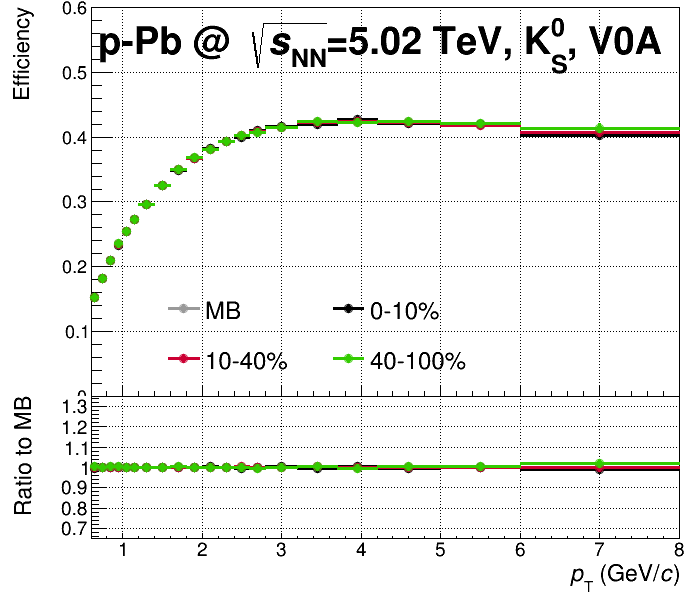
\includegraphics[width=.32\textwidth]{c04V0Reconstruction/cKshort_Efficiency}
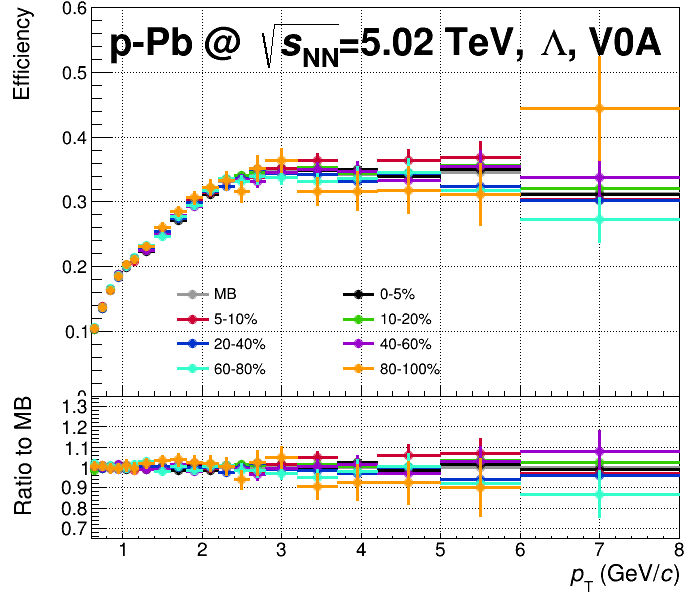
\includegraphics[width=.32\textwidth]{c04V0Reconstruction/cLambda_Efficiency}
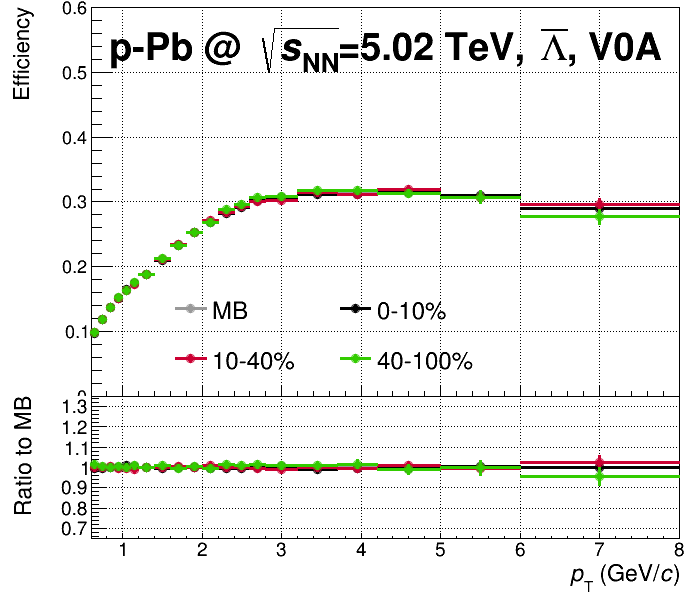
\includegraphics[width=.32\textwidth]{c04V0Reconstruction/cAntiLa_Efficiency}
\caption{Efficiency of inclusive $\Vzeros$ as a function of $\pT$ in three event multiplicity bins with V0A centrality estimator.}
\label{fig:c05EffiIncV0s}
\end{center}
\end{figure}

Due to differences in the experimental acceptance for \Vzero\ particles associated to jets (JC) and those extracted through the various estimators (OC, PC, NJ) of the underlying event the efficiencies of \Vzero\ particles were estimated separately in every case.

%%%%%%%%%%%%%%%%%%%%%%%%%%%%%%%%%%%%%%%%%%%%%%%%%%%%%%%%%%%%%%%%%%
\subsection{Feed-down subtraction for \lda\ and \alda}

The \pt\ differential yields of \lda\ and \alda\ reconstructed for each selection (JC and UE selections) where corrected for the feed-down from $\Xi$ decays. 
%%The correction was applied before the efficiency corrections. 
The $\Xi$ production in jets (JC) was estimated based on measurements of the multi-strange baryons and their decays at high-\pt\ performed in \pp\ collisions \cite{Abelev:2012jp} and extrapolated to the lower \pt\ using PYTHIA event generator and full detector simulations.
